\begin{center}
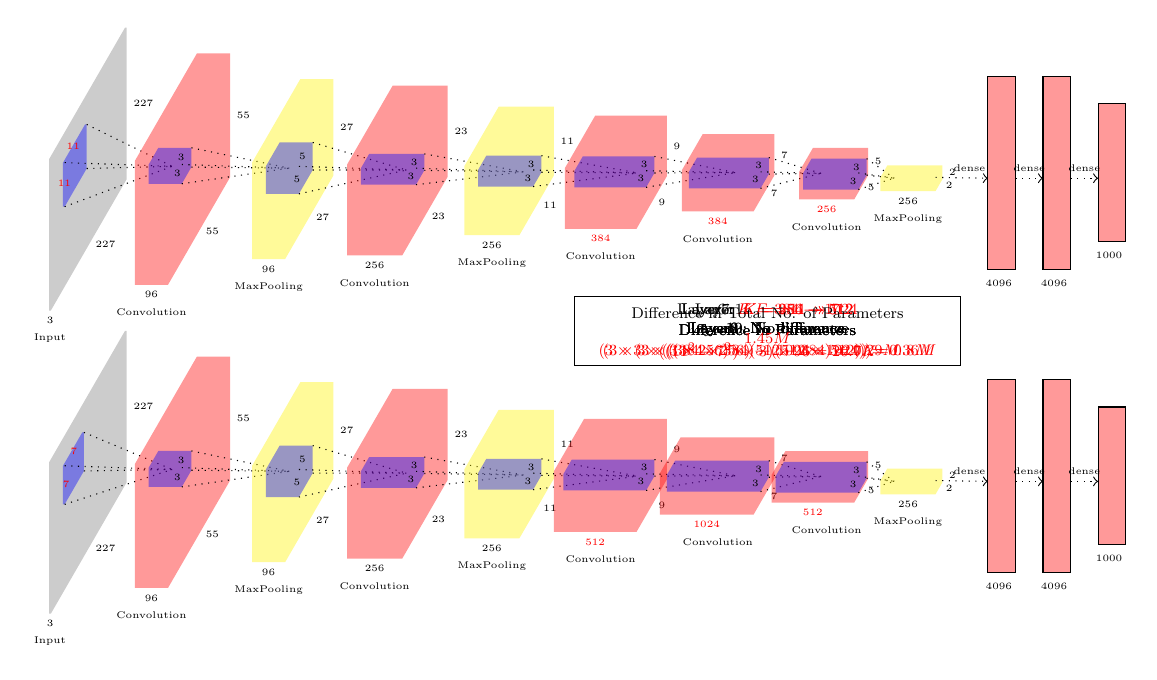
\begin{tikzpicture}[scale=0.7,transform shape]

\pgfsetxvec{\pgfpoint{1cm}{0cm}}
\pgfsetyvec{\pgfpoint{0cm}{0.5*1cm}}
\pgfsetzvec{\pgfpoint{0.5*-.5cm}{0.5*-.866cm}}

\def\cuboid#1#2#3#4#5{
\begin{scope}
\edef\mycolor{#2}
\edef\depth{#3}
\edef\height{#4}
\edef\width{#5}
\draw[black,fill=\mycolor, fill opacity=0.4, text opacity=1] #1 -- ++(-\depth,0,0) -- ++(0,-\height,0) -- ++(\depth,0,0) -- cycle #1 -- ++(0,0,-\width) -- ++(0,-\height,0) -- ++(0,0,\width) -- cycle  #1 -- ++(-\depth,0,0) -- ++(0,0,-\width) -- ++(\depth,0,0) -- cycle;
\end{scope}
}

\def\cuboidlabeldiff#1#2#3#4#5#6#7#8{
\begin{scope}
\edef\mycolor{#2}
\edef\depth{#3}
\edef\height{#4}
\edef\width{#5}
\edef\depthlabel{#6}
\edef\heightlabel{#7}
\edef\widthlabel{#8}
\draw[draw=none,fill=\mycolor, fill opacity=0.4, text opacity=1] #1 -- ++(-\depth,0,0) -- ++(0,-\height,0) -- ++(\depth,0,0) node[red,pos=0.5,below] {\tiny \depthlabel} -- cycle #1 -- ++(0,0,-\width) -- ++(0,-\height,0) node[black,pos=0.5,right] {\tiny \heightlabel} -- ++(0,0,\width)  node[black,pos=0.5,below,right] {\tiny \widthlabel} -- cycle  #1 -- ++(-\depth,0,0) -- ++(0,0,-\width) -- ++(\depth,0,0) -- cycle;
\end{scope}
}
\def\cuboidlabel#1#2#3#4#5#6#7#8{
\begin{scope}
\edef\mycolor{#2}
\edef\depth{#3}
\edef\height{#4}
\edef\width{#5}
\edef\depthlabel{#6}
\edef\heightlabel{#7}
\edef\widthlabel{#8}
\draw[draw=none,fill=\mycolor, fill opacity=0.4, text opacity=1] #1 -- ++(-\depth,0,0) -- ++(0,-\height,0) -- ++(\depth,0,0) node[black,pos=0.5,below] {\tiny \depthlabel} -- cycle #1 -- ++(0,0,-\width) -- ++(0,-\height,0) node[black,pos=0.5,right] {\tiny \heightlabel} -- ++(0,0,\width)  node[black,pos=0.5,below,right] {\tiny \widthlabel} -- cycle  #1 -- ++(-\depth,0,0) -- ++(0,0,-\width) -- ++(\depth,0,0) -- cycle;
\end{scope}
}

\def\kernellabeldiff#1#2#3#4#5#6#7#8#9{
%#6 is target pixel
\begin{scope}
\edef\mycolor{#2}
\edef\depth{#3}
\edef\height{#4}
\edef\width{#5}
\edef\depthlabel{#7}
\edef\heightlabel{#8}
\edef\widthlabel{#9}
\draw[draw=none,fill=\mycolor, fill opacity=0.4, text opacity=1] #1 -- ++(-\depth,0,0) -- ++(0,-\height,0) -- ++(\depth,0,0) -- cycle #1 -- ++(0,0,-\width) -- ++(0,-\height,0) node[red,pos=0.5,left] {\tiny \heightlabel} -- ++(0,0,\width)  node[red,pos=0.4,above,left] {\tiny \widthlabel} -- cycle  #1 -- ++(-\depth,0,0) -- ++(0,0,-\width) -- ++(\depth,0,0) -- cycle;

\draw[dotted] #1 -- #6 #1++(0,0,-\width) -- #6 #1++(0,-\height,0) -- #6 #1++(0,-\height,-\width) -- #6;

\end{scope}
}

\def\kernellabel#1#2#3#4#5#6#7#8#9{
%#6 is target pixel
\begin{scope}
\edef\mycolor{#2}
\edef\depth{#3}
\edef\height{#4}
\edef\width{#5}
\edef\depthlabel{#7}
\edef\heightlabel{#8}
\edef\widthlabel{#9}
\draw[draw=none,fill=\mycolor, fill opacity=0.4, text opacity=1] #1 -- ++(-\depth,0,0) -- ++(0,-\height,0) -- ++(\depth,0,0) -- cycle #1 -- ++(0,0,-\width) -- ++(0,-\height,0) node[pos=0.5,left] {\tiny \heightlabel} -- ++(0,0,\width)  node[pos=0.4,above,left] {\tiny \widthlabel} -- cycle  #1 -- ++(-\depth,0,0) -- ++(0,0,-\width) -- ++(\depth,0,0) -- cycle;

\draw[dotted] #1 -- #6 #1++(0,0,-\width) -- #6 #1++(0,-\height,0) -- #6 #1++(0,-\height,-\width) -- #6;

\end{scope}
}


\edef\zfshift{11}
\cuboid{(16.5,6-\zfshift,0)}{white}{7}{2.5}{0}{256}{2}{2}
%alexnet
%input
\onslide<1->{
\cuboidlabel{(0,0,0)}{gray}{0.03}{5.5}{5.5}{3}{227}{227}
\cuboidlabel{(0,-\zfshift,0)}{gray}{0.03}{5.5}{5.5}{3}{227}{227}
\node (a) at (-0.015,-6.5,0) {\tiny Input};
\node (a) at (-0.015,-6.5-\zfshift,0) {\tiny Input};
}
\onslide<2->{
\kernellabeldiff{(0,-1,-1)}{blue}{0.03}{1.6}{1.6}{(1.7,-2,-2)}{3}{11}{11}
\kernellabeldiff{(0,-1-\zfshift,-1)}{blue}{0.03}{1.4}{1.4}{(1.7,-2-\zfshift,-2)}{3}{7}{7}
}

\onslide<2-3>{
\node (a) at (16.5-7*0.5,6-\zfshift-0.5,0) {\footnotesize Layer1: \color{red}{$F=11 \to 7$}};
\node (a) at (16.5-7*0.5,6-\zfshift-1.2,0) {\footnotesize Difference in Parameters};
\node (a) at (16.5-7*0.5,6-\zfshift-2,0) {\footnotesize \color{red}{$((11^2-7^2)\times 3) \times 96 = 20.7K$}};
}


\onslide<3->{
\cuboidlabel{(2,-0.5,-0.5)}{red}{0.6}{4.5}{4.5}{96}{55}{55}
\cuboidlabel{(2,-0.5-\zfshift,-0.5)}{red}{0.6}{4.5}{4.5}{96}{55}{55}
\node (a) at (2-0.3,-0.5-4.5-1,-0.5) {\tiny Convolution};
\node (a) at (2-0.3,-0.5-4.5-1-\zfshift,-0.5) {\tiny Convolution};
}
\onslide<4->{
\kernellabel{(2,-1.5,-1.5)}{blue}{0.6}{0.7}{0.7}{(3.7,-2.5,-2.5)}{96}{3}{3}
\kernellabel{(2,-1.5-\zfshift,-1.5)}{blue}{0.6}{0.7}{0.7}{(3.7,-2.5-\zfshift,-2.5)}{96}{3}{3}
}

\onslide<4-5>{
\node (a) at (16.5-7*0.5,6-\zfshift-1.2,0) {\footnotesize Layer2: No difference};
}

\onslide<5->{
\cuboidlabel{(4,-1,-1)}{yellow}{0.6}{3.5}{3.5}{96}{27}{27}
\cuboidlabel{(4,-1-\zfshift,-1)}{yellow}{0.6}{3.5}{3.5}{96}{27}{27}
\node (a) at (4-0.3,-1-3.5-1,-1) {\tiny MaxPooling};
\node (a) at (4-0.3,-1-3.5-1-\zfshift,-1) {\tiny MaxPooling};
}
\onslide<6->{
\kernellabel{(4,-2,-2)}{blue}{0.6}{1}{1}{(5.7,-3,-3)}{96}{5}{5}
\kernellabel{(4,-2-\zfshift,-2)}{blue}{0.6}{1}{1}{(5.7,-3-\zfshift,-3)}{96}{5}{5}
}
\onslide<6-7>{
\node (a) at (16.5-7*0.5,6-\zfshift-1.2,0) {\footnotesize Layer3: No difference};
}


\onslide<7->{
\cuboidlabel{(6,-1.5,-1.5)}{red}{1}{3.3}{3.3}{256}{23}{23}
\cuboidlabel{(6,-1.5-\zfshift,-1.5)}{red}{1}{3.3}{3.3}{256}{23}{23}
\node (a) at (6-0.5,-1.5-3.3-1,-1.5) {\tiny Convolution};
\node (a) at (6-0.5,-1.5-3.3-1-\zfshift,-1.5) {\tiny Convolution};
}
\onslide<8->{
\kernellabel{(6,-2.5,-2.5)}{blue}{1}{0.6}{0.6}{(7.7,-3.5,-3.5)}{256}{3}{3}
\kernellabel{(6,-2.5-\zfshift,-2.5)}{blue}{1}{0.6}{0.6}{(7.7,-3.5-\zfshift,-3.5)}{256}{3}{3}
}
\onslide<8-9>{
\node (a) at (16.5-7*0.5,6-\zfshift-1.2,0) {\footnotesize Layer4: No difference};
}

\onslide<9->{
\cuboidlabel{(8,-2,-2)}{yellow}{1}{2.5}{2.5}{256}{11}{11}
\cuboidlabel{(8,-2-\zfshift,-2)}{yellow}{1}{2.5}{2.5}{256}{11}{11}
\node (a) at (8-0.5,-2-2.5-1,-2) {\tiny MaxPooling};
\node (a) at (8-0.5,-2-2.5-1-\zfshift,-2) {\tiny MaxPooling};
}
\onslide<10->{
\kernellabel{(8,-3,-3)}{blue}{1}{0.6}{0.6}{(9.7,-3.8,-3.8)}{256}{3}{3}
\kernellabel{(8,-3-\zfshift,-3)}{blue}{1}{0.6}{0.6}{(9.7,-3.8-\zfshift,-3.8)}{256}{3}{3}
}

\onslide<10-11>{
\node (a) at (16.5-7*0.5,6-\zfshift-0.5,0) {\footnotesize Layer5: \color{red}{$K = 384 \to 512$}};
\node (a) at (16.5-7*0.5,6-\zfshift-1.2,0) {\footnotesize Difference in Parameters};
\node (a) at (16.5-7*0.5,6-\zfshift-2,0) {\footnotesize \color{red}{$(3 \times 3 \times 256) \times (512-384) = 0.29M$}};
}


\onslide<11->{
\cuboidlabeldiff{(10,-2.5,-2.5)}{red}{1.3}{2.2}{2.2}{384}{9}{9}
\cuboidlabeldiff{(10,-2.5-\zfshift,-2.5)}{red}{1.5}{2.2}{2.2}{512}{9}{9}
\node (a) at (10-0.65,-2.5-2.2-1,-2.5) {\tiny Convolution};
\node (a) at (10-0.65,-2.5-2.2-1-\zfshift,-2.5) {\tiny Convolution};
}
\onslide<12->{
\kernellabel{(10,-3.2,-3.2)}{blue}{1.3}{0.6}{0.6}{(11.5,-3.7,-3.7)}{384}{3}{3}
\kernellabel{(10,-3.2-\zfshift,-3.2)}{blue}{1.5}{0.6}{0.6}{(11.5,-3.7-\zfshift,-3.7)}{512}{3}{3}
}

\onslide<12-13>{
\node (a) at (16.5-7*0.5,6-\zfshift-0.5,0) {\footnotesize Layer6: \color{red}{$K = 384 \to 1024$}};
\node (a) at (16.5-7*0.5,6-\zfshift-1.2,0) {\footnotesize Difference in Parameters};
\node (a) at (16.5-7*0.5,6-\zfshift-2,0) {\footnotesize \color{red}{$(3 \times 3 \times ((384 \times 384) - (512 \times 1024)) = 0.8M$}};
}

\onslide<13->{
\cuboidlabeldiff{(12,-3,-3)}{red}{1.3}{1.5}{1.5}{384}{7}{7}
\cuboidlabeldiff{(12,-3-\zfshift,-3)}{red}{1.7}{1.5}{1.5}{1024}{7}{7}
\node (a) at (12-0.65,-3-1.5-1,-3) {\tiny Convolution};
\node (a) at (12-0.65,-3-1.5-1-\zfshift,-3) {\tiny Convolution};
}
\onslide<14->{
\kernellabel{(12,-3.5,-3.5)}{blue}{1.3}{0.6}{0.6}{(13,-3.9,-3.9)}{384}{3}{3}
\kernellabel{(12,-3.5-\zfshift,-3.5)}{blue}{1.7}{0.6}{0.6}{(13,-3.9-\zfshift,-3.9)}{1024}{3}{3}
}

\onslide<14-15>{
\node (a) at (16.5-7*0.5,6-\zfshift-0.5,0) {\footnotesize Layer7: \color{red}{$K = 256 \to 512$}};
\node (a) at (16.5-7*0.5,6-\zfshift-1.2,0) {\footnotesize Difference in Parameters};
\node (a) at (16.5-7*0.5,6-\zfshift-2,0) {\footnotesize \color{red}{$(3 \times 3 \times ((384 \times 256) - (1024 \times 512)) = 0.36M$}};
}

\onslide<15->{
\cuboidlabeldiff{(13.7,-3.5,-3.5)}{red}{1}{1}{1}{256}{5}{5}
\cuboidlabeldiff{(13.7,-3.5-\zfshift,-3.5)}{red}{1.5}{1}{1}{512}{5}{5}
\node (a) at (13.7-0.5,-3.5-1-1,-3.5) {\tiny Convolution};
\node (a) at (13.7-0.5,-3.5-1-1-\zfshift,-3.5) {\tiny Convolution};
}
\onslide<16->{
\kernellabel{(13.7,-3.8,-3.8)}{blue}{1}{0.6}{0.6}{(14,-5.2,-5.2)}{256}{3}{3}
\kernellabel{(13.7,-3.8-\zfshift,-3.8)}{blue}{1.5}{0.6}{0.6}{(14,-5.2-\zfshift,-5.2)}{512}{3}{3}
}

\onslide<16-17>{
\node (a) at (16.5-7*0.5,6-\zfshift-1.2,0) {\footnotesize Layer8: No difference};
}


\onslide<17->{
\cuboidlabel{(14.8,-5,-5)}{yellow}{1}{0.5}{0.5}{256}{2}{2}
\cuboidlabel{(14.8,-5-\zfshift,-5)}{yellow}{1}{0.5}{0.5}{256}{2}{2}
\node (a) at (14.8-0.5,-5-0.5-1,-5) {\tiny MaxPooling};
\node (a) at (14.8-0.5,-5-0.5-1-\zfshift,-5) {\tiny MaxPooling};
}
\onslide<18>{
\node (a) at (16.5-7*0.5,6-\zfshift-1.2,0) {\footnotesize Layer9: No difference};
}

\onslide<18->{
\draw[dotted,->] (14.8,-5,-5) -- (17,-0.7,0) node[pos=0.65,above] {\tiny dense};
\cuboid{(17.5,3,0)}{red}{0.5}{7}{0}{256}{2}{2}
\node (a) at (17.2,-4.5,0) {\tiny 4096};

\draw[dotted,->] (14.8,-5-\zfshift,-5) -- (17,-0.7-\zfshift,0) node[pos=0.65,above] {\tiny dense};
\cuboid{(17.5,3-\zfshift,0)}{red}{0.5}{7}{0}{256}{2}{2}
\node (a) at (17.2,-4.5-\zfshift,0) {\tiny 4096};
}

\onslide<19>{
\node (a) at (16.5-7*0.5,6-\zfshift-1.2,0) {\footnotesize Layer10: No difference};
}

\onslide<19->{
\draw[dotted,->] (17.5,-0.7,0) -- (18,-0.7,0) node[pos=0.5,above] {\tiny dense};
\cuboid{(18.5,3,0)}{red}{0.5}{7}{0}{256}{2}{2}
\node (a) at (18.2,-4.5,0) {\tiny 4096};

\draw[dotted,->] (17.5,-0.7-\zfshift,0) -- (18,-0.7-\zfshift,0) node[pos=0.5,above] {\tiny dense};
\cuboid{(18.5,3-\zfshift,0)}{red}{0.5}{7}{0}{256}{2}{2}
\node (a) at (18.2,-4.5-\zfshift,0) {\tiny 4096};
}

\onslide<20>{
\node (a) at (16.5-7*0.5,6-\zfshift-1.2,0) {\footnotesize Layer10: No difference};
}


\onslide<20->{
\draw[dotted,->] (18.5,-0.7,0) -- (19,-0.7,0) node[pos=0.5,above] {\tiny dense};
\cuboid{(19.5,2,0)}{red}{0.5}{5}{0}{256}{2}{2}
\node (a) at (19.2,-3.5,0) {\tiny 1000};

\draw[dotted,->] (18.5,-0.7-\zfshift,0) -- (19,-0.7-\zfshift,0) node[pos=0.5,above] {\tiny dense};
\cuboid{(19.5,2-\zfshift,0)}{red}{0.5}{5}{0}{256}{2}{2}
\node (a) at (19.2,-3.5-\zfshift,0) {\tiny 1000};
}

\onslide<21>{
\node (a) at (16.5-7*0.5,6-\zfshift-0.6,0) {\footnotesize Difference in Total No. of Parameters};
\node (a) at (16.5-7*0.5,6-\zfshift-1.5,0) {\footnotesize \color{red}{$1.45M$}};
}

\end{tikzpicture}
\end{center}

